\documentclass[aspectratio=169]{beamer} % dvipsnames gives more built-in colors
\usepackage{graphicx} % Required for inserting images
\usepackage{transparent}
\usepackage{float}
\usepackage{tikz}
\usepackage{amsmath}
\usepackage[font=scriptsize,labelfont=bf]{caption}
\usepackage{algorithmicx}
\usepackage{listings}
\usepackage{animate}
\renewcommand{\footnotesize}{\tiny}

\usepackage{tikz}
\usepackage{tikz-cd}

\usepackage{babel}  
\usepackage{siunitx}  
\sisetup{locale = DE}
\usepackage{multicol}
\usepackage{listings}

\usetikzlibrary{arrows.meta, angles, quotes, calc}

%\usepackage[sorting=none]{biblatex}
\usepackage[german=guillemets]{csquotes}
\setquotestyle{english}
%\addbibresource{bibliography.bib}

\usetheme{ufr}
\usecolortheme{ufr}


\title{What you needa know about Yoneda}
\author{Emma Bach (she/her)}
\date{Seminar on Functional Programming and Logic, Summer Semester 2025}

\begin{document}

{
\usebackgroundtemplate{
        \transparent{0.1}    
        \hspace{7cm}
        
\includegraphics[width=0.7\paperwidth]{logos/ufr-siegel-grey.png}
        }

\begin{frame}[plain]
    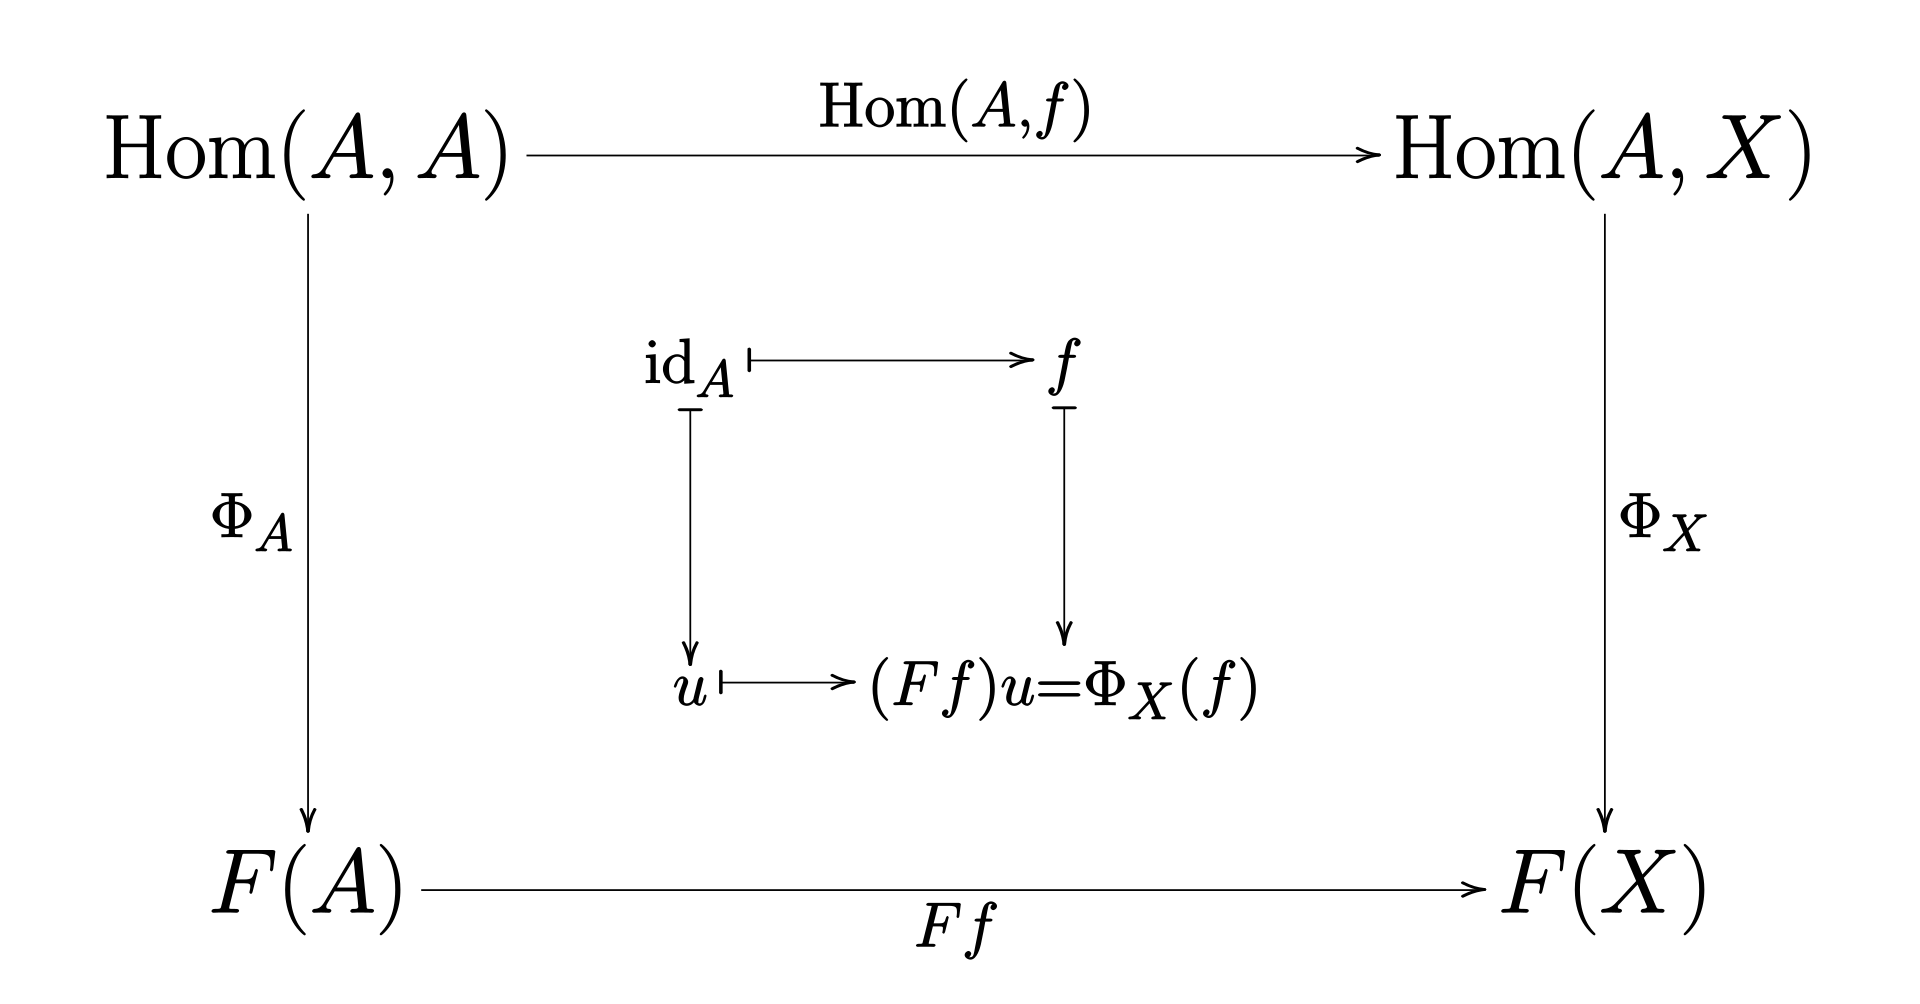
\includegraphics[width=0.4\paperwidth]{figures/Yoneda_lemma_cd.svg.png}
    \titlepage
\end{frame}

\begin{frame}{Motivation}
 \begin{itemize}
  \item A common sentiment in many cultures is the idea that people are defined by how they interact with their surroundings.
  \item ``\textit{Tell me your company, and I will tell you what you are.}''\footnote{Quoted as a proverb in \textit{Don Quixote}}
  \item The Yoneda Lemma is the result of applying this way of thinking to mathematical objects within the extremely general setting of \textit{Category Theory}.
 \end{itemize}

\end{frame}

\begin{frame}{Categories}
\begin{columns}
\column{0.5\textwidth}
A \textit{category} is defined as a class of \textit{objects} together with a class of \textit{morphisms} (sometimes called \textit{arrows})
\begin{itemize}
 \item Each morphism $f : A \to B$ relates some \textit{source} object $A$ to some \textit{target} object $B$.
 \item Two morphisms $f: A \to B$ and $g : B \to C$ can be composed into a morphism $g \circ f : A \to C$
 \item $h \circ (g \circ f) = (h \circ g) \circ f$ (Composition is associative)
 \item $
\end{itemize}
\column{0.5\textwidth}
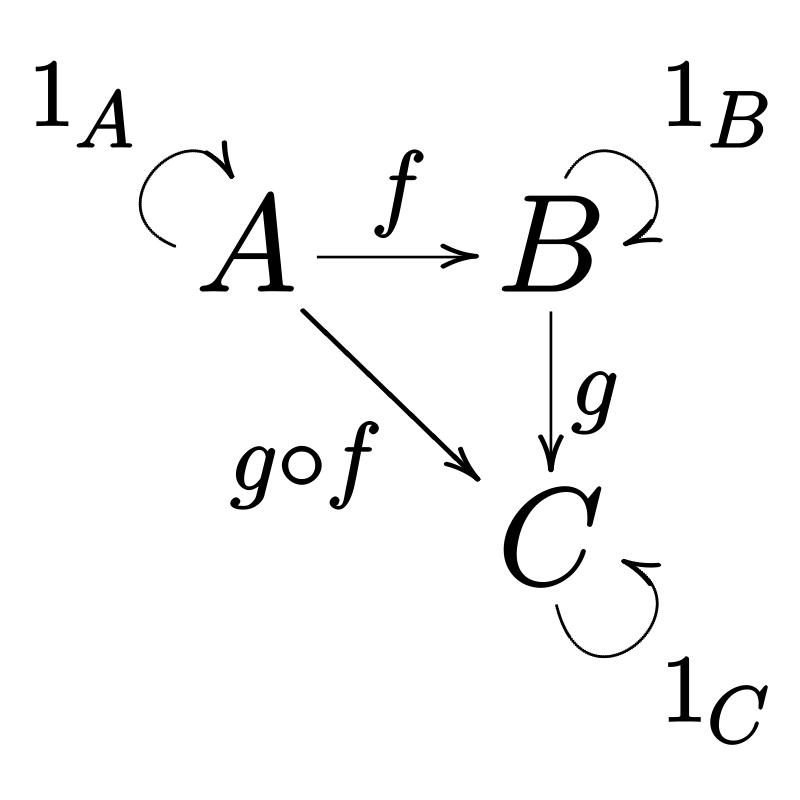
\includegraphics[width=0.5\textwidth]{figures/category.png}
\end{columns}
\end{frame}

}

\end{document}
